\begin{frame}
  \begin{center}
    {\Large Why do we need multiple layers?}
  \end{center}
\end{frame}

\begin{frame}
  \begin{center}
    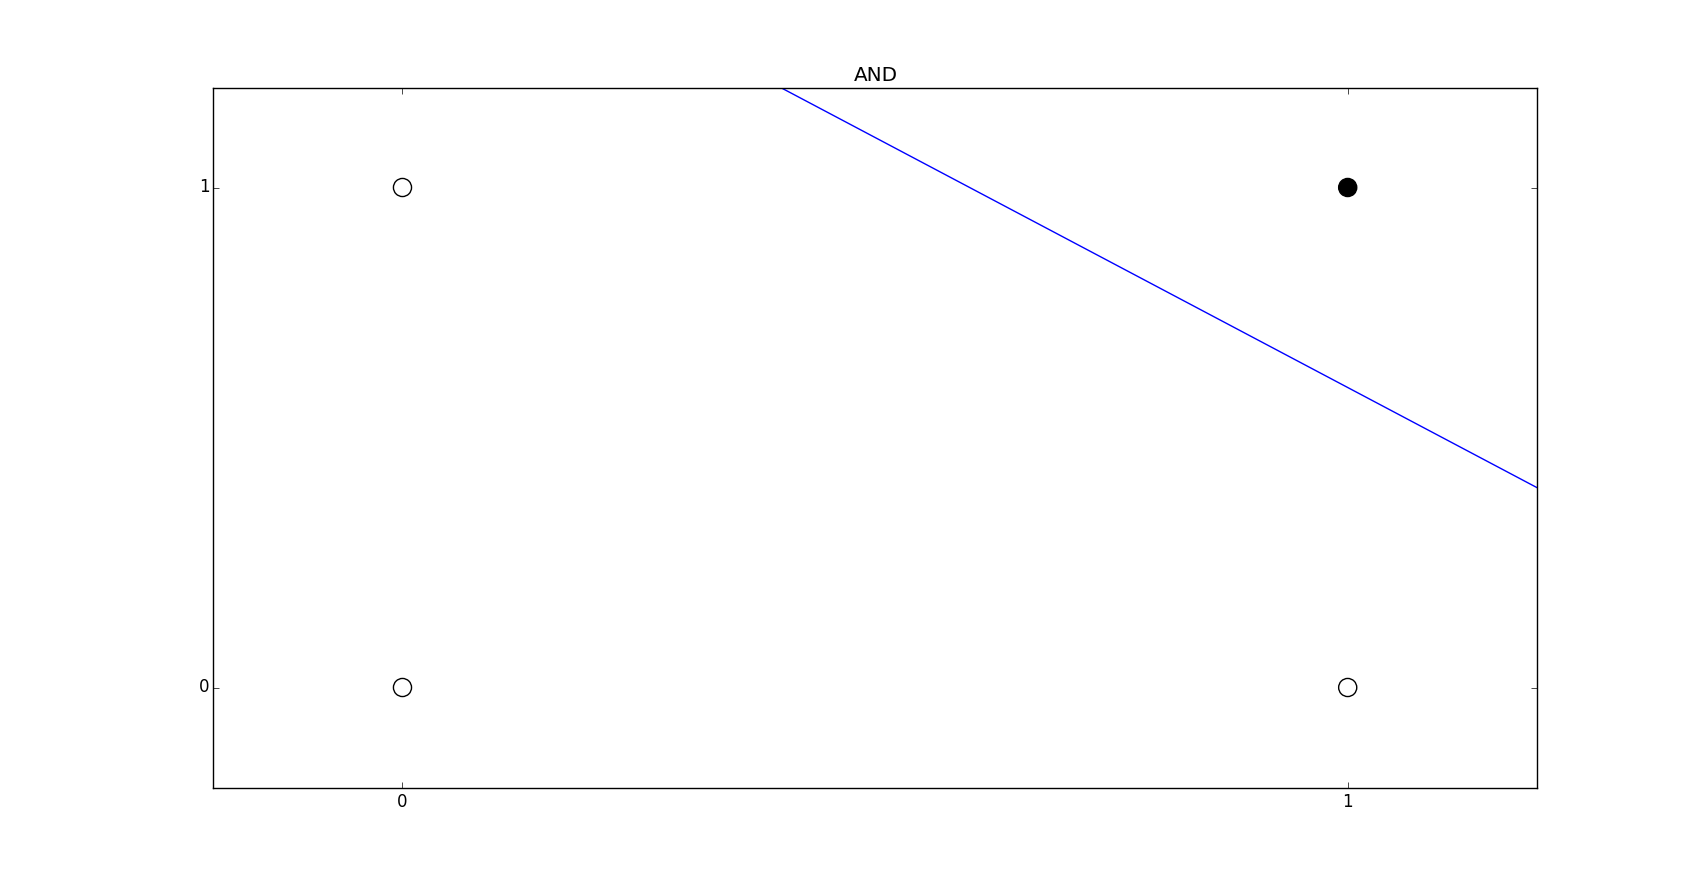
\includegraphics[scale=0.25]{pictures/and.png}
  \end{center}
\end{frame}

\begin{frame}
  \begin{center}
    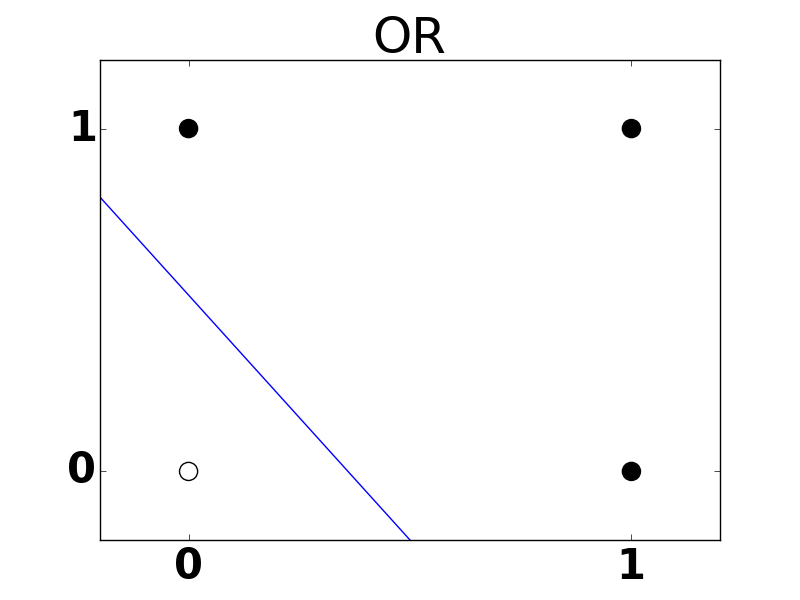
\includegraphics[scale=0.25]{pictures/or.png}
  \end{center}
\end{frame}

\begin{frame}
  \begin{center}
    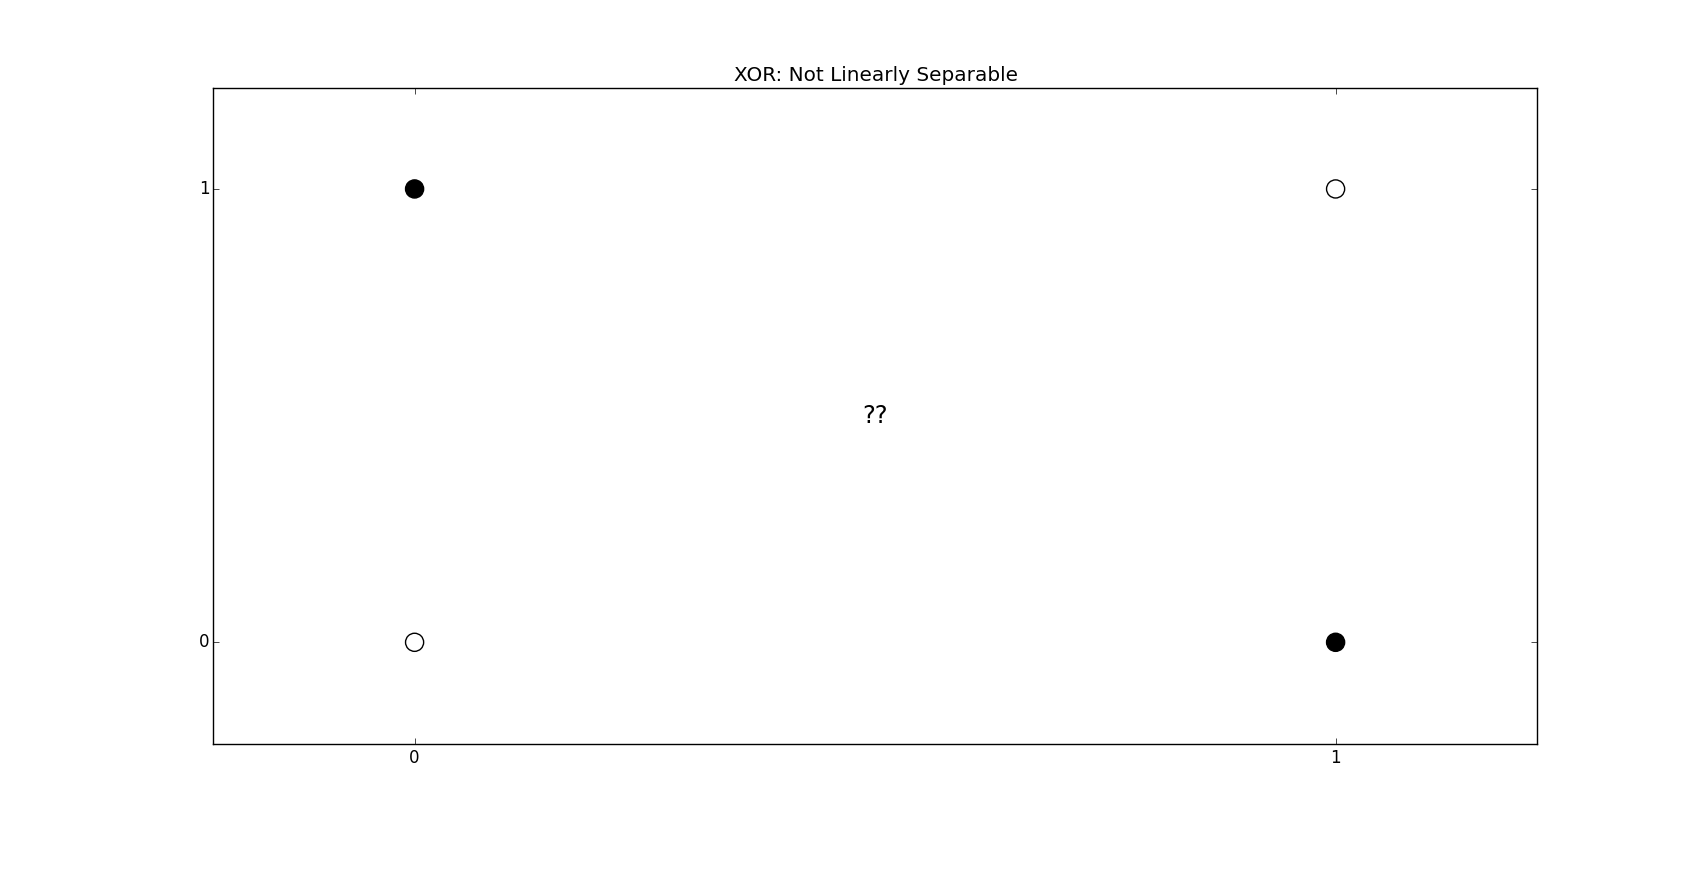
\includegraphics[scale=0.25]{pictures/xor.png}
  \end{center}
\end{frame}

\begin{frame}[fragile]
  \begin{block}{Forward propagation}
    \begin{lstlisting}
def h(x, w):
    out = [x]
    for l in range(len(w)):
        x = insert(out[l], 0, 1, axis=0)
        o = g(transpose(w[l]) * x)
        out.append(o)
    return out
  \end{lstlisting}
  \end{block}
\end{frame}
% Linearly separable data vs non-linearly separable data.

% if input is (x1, x2), add x1^2, x2^2 and x1x2 as inputs
